\section{Decomposition view (UML Component diagram)}\label{sec:decomposition}
Discuss the decompositions of the components of the client-server view which
you have further decomposed.

\subsection{AuthenticableUserManager}
\begin{figure}[!htp]
    \centering
    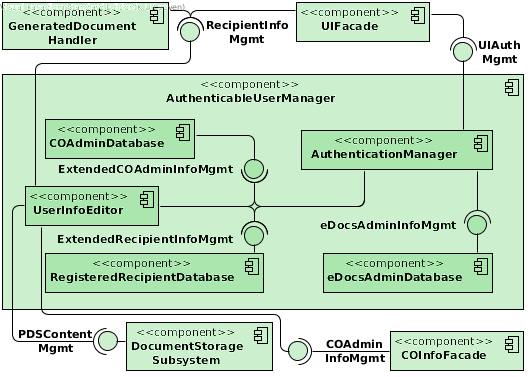
\includegraphics[width=\textwidth]{figures/AuthenticableUserManager.png}
    \caption{Decomposition of \texttt{AuthenticableUserManager}}\label{fig:decomp-authuserman}
\end{figure}

Describe the decomposition of \texttt{ComponentX} and how this relates to the
requirements.

\subsection{BillingSubsystem}
\begin{figure}[!htp]
    \centering
    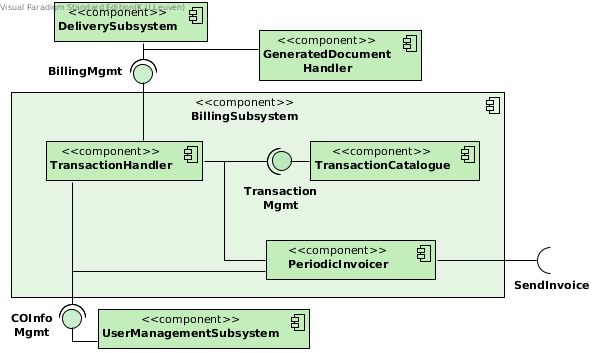
\includegraphics[width=\textwidth]{figures/Billing Subsystem.png}
    \caption{Decomposition of \texttt{BillingSubsystem}}\label{fig:decomp-billingsub}
\end{figure}

Describe the decomposition of \texttt{ComponentX} and how this relates to the
requirements.

\subsection{CommunicationSubsystem}
\begin{figure}[!htp]
    \centering
    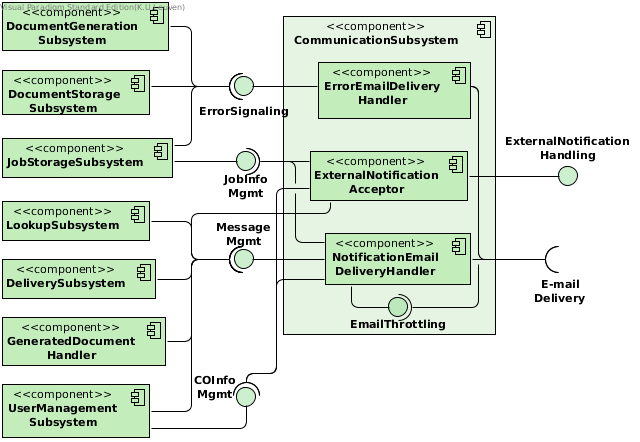
\includegraphics[width=\textwidth]{figures/Communication Subsystem.png}
    \caption{Decomposition of \texttt{CommunicationSubsystem}}\label{fig:decomp-commsub}
\end{figure}

Describe the decomposition of \texttt{ComponentX} and how this relates to the
requirements.

\subsection{DeliverySubsystem}
\begin{figure}[!htp]
    \centering
    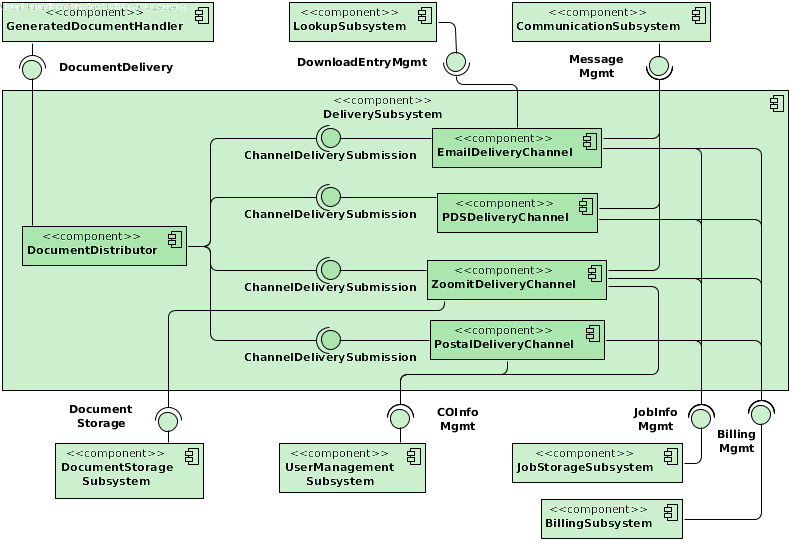
\includegraphics[width=\textwidth]{figures/Delivery Subsystem.png}
    \caption{Decomposition of \texttt{DeliverySubsystem}}\label{fig:decomp-delisub}
\end{figure}

Describe the decomposition of \texttt{ComponentX} and how this relates to the
requirements.

\subsection{DocumentGenerationSubsystem}
\begin{figure}[!htp]
    \centering
    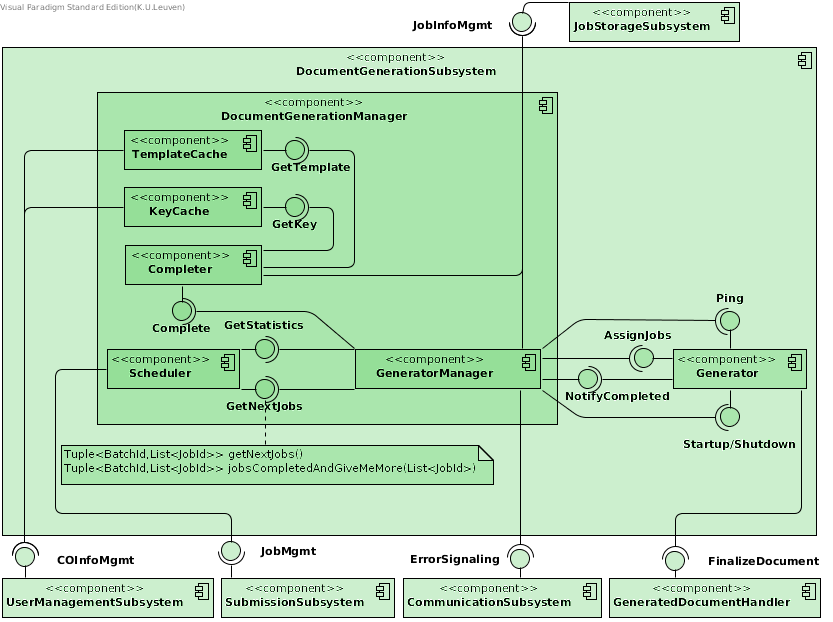
\includegraphics[width=\textwidth]{figures/Document Generation Subsystem.png}
    \caption{Decomposition of \texttt{DocumentGenerationSubsystem}}\label{fig:decomp-docgensub}
\end{figure}

Describe the decomposition of \texttt{ComponentX} and how this relates to the
requirements.

\subsection{DocumentStorageSubsystem}
\begin{figure}[!htp]
    \centering
    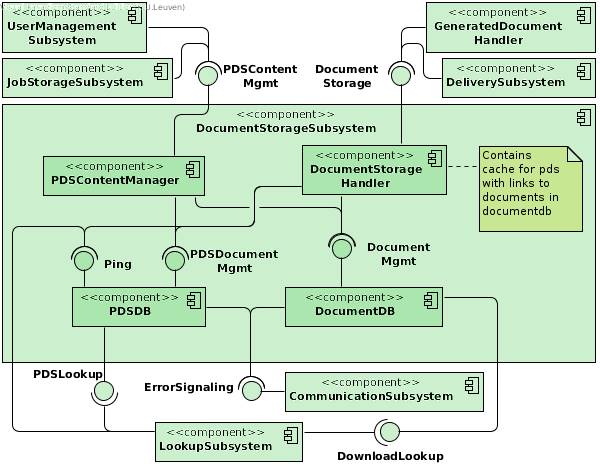
\includegraphics[width=\textwidth]{figures/Document Storage Subsystem.png}
    \caption{Decomposition of \texttt{DocumentStorageSubsystem}}\label{fig:decomp-docstosub}
\end{figure}

Describe the decomposition of \texttt{ComponentX} and how this relates to the
requirements.

\subsection{DocumentStorageHandler}
\begin{figure}[!htp]
    \centering
    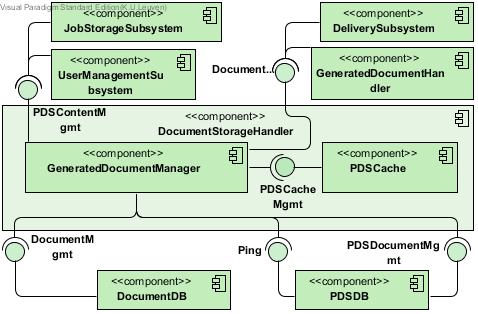
\includegraphics[width=\textwidth]{figures/DocumentStorageHandler.png}
    \caption{Decomposition of \texttt{DocumentStorageHandler}}\label{fig:decomp-docstohan}
\end{figure}

Describe the decomposition of \texttt{ComponentX} and how this relates to the
requirements.

\subsection{DocumentDB}
\begin{figure}[!htp]
    \centering
    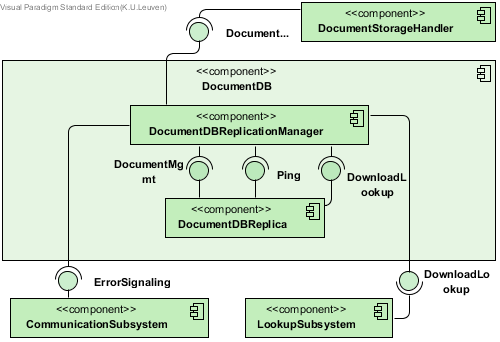
\includegraphics[width=\textwidth]{figures/DocumentDB.png}
    \caption{Decomposition of \texttt{DocumentDB}}\label{fig:decomp-docdb}
\end{figure}

Describe the decomposition of \texttt{ComponentX} and how this relates to the
requirements.

\subsection{PDSDB}
\begin{figure}[!htp]
    \centering
    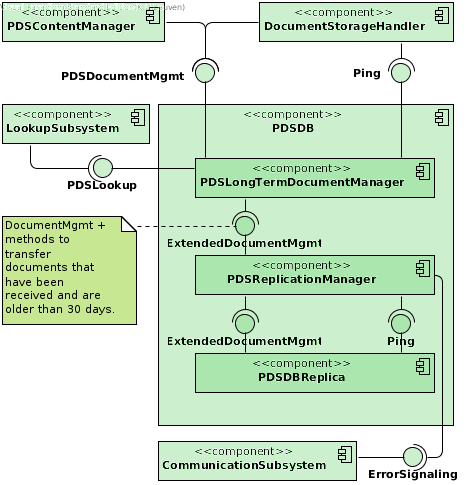
\includegraphics[width=\textwidth]{figures/PDSDB.png}
    \caption{Decomposition of \texttt{PDSDB}}\label{fig:decomp-pdsdb}
\end{figure}

Describe the decomposition of \texttt{ComponentX} and how this relates to the
requirements.

\subsection{JobStorageSubsystem}
\begin{figure}[!htp]
    \centering
    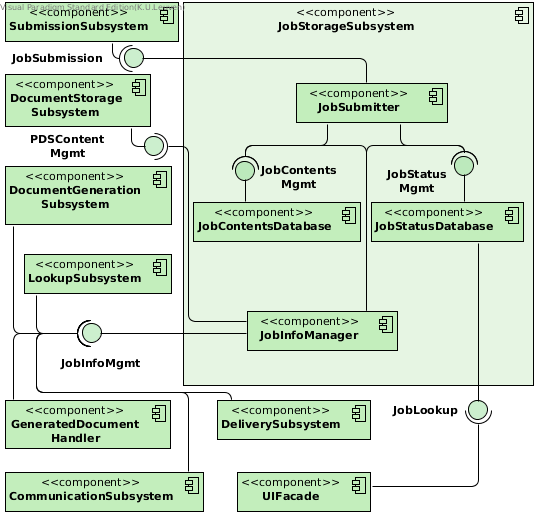
\includegraphics[width=\textwidth]{figures/Job Storage Subsystem.png}
    \caption{Decomposition of \texttt{JobStorageSubsystem}}\label{fig:decomp-jobsub}
\end{figure}

Describe the decomposition of \texttt{ComponentX} and how this relates to the
requirements.

\subsection{LookupSubsystem}
\begin{figure}[!htp]
    \centering
    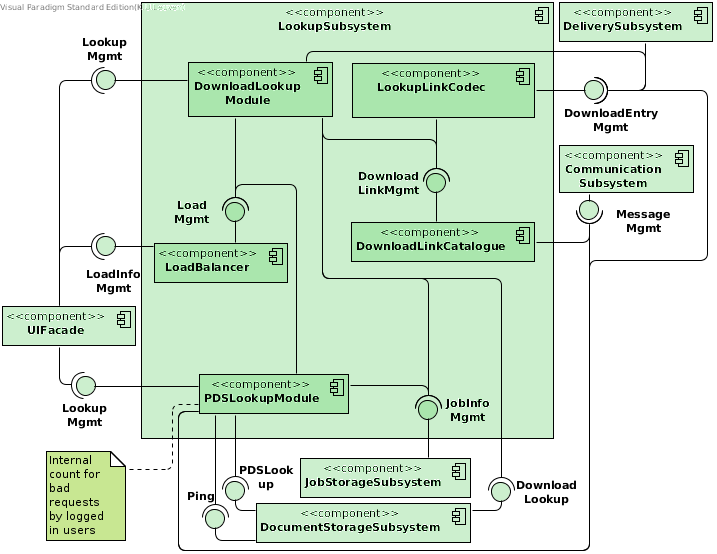
\includegraphics[width=\textwidth]{figures/Lookup Subsystem.png}
    \caption{Decomposition of \texttt{LookupSubsystem}}\label{fig:decomp-lookupsub}
\end{figure}

Describe the decomposition of \texttt{ComponentX} and how this relates to the
requirements.

\subsection{SubmissionSubsystem}
\begin{figure}[!htp]
    \centering
    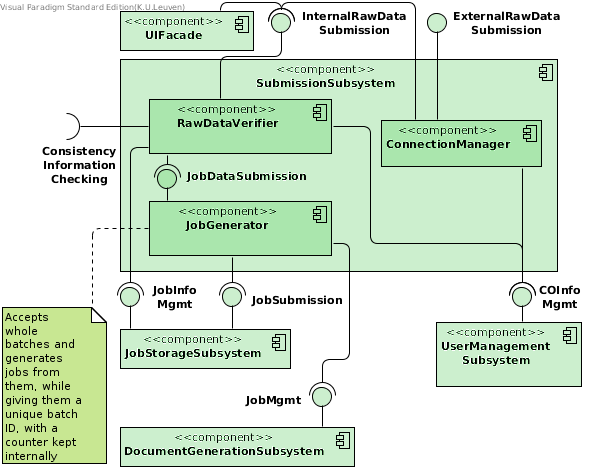
\includegraphics[width=\textwidth]{figures/Submission Subsystem.png}
    \caption{Decomposition of \texttt{SubmissionSubsystem}}\label{fig:decomp-submsub}
\end{figure}

Describe the decomposition of \texttt{ComponentX} and how this relates to the
requirements.

\subsection{UIFacade}
\begin{figure}[!htp]
    \centering
    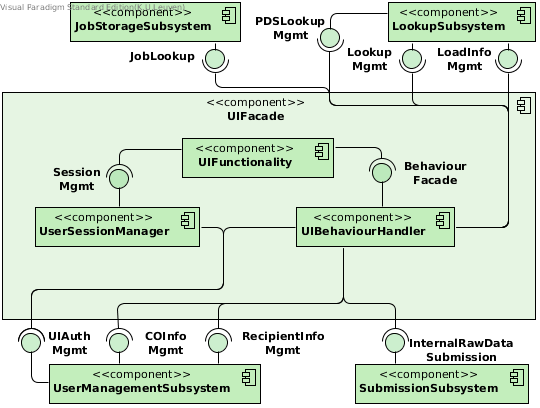
\includegraphics[width=\textwidth]{figures/UI Facade.png}
    \caption{Decomposition of \texttt{UIFacade}}\label{fig:decomp-uif}
\end{figure}

Describe the decomposition of \texttt{ComponentX} and how this relates to the
requirements.

\subsection{UserManagementSubsystem}
\begin{figure}[!htp]
    \centering
    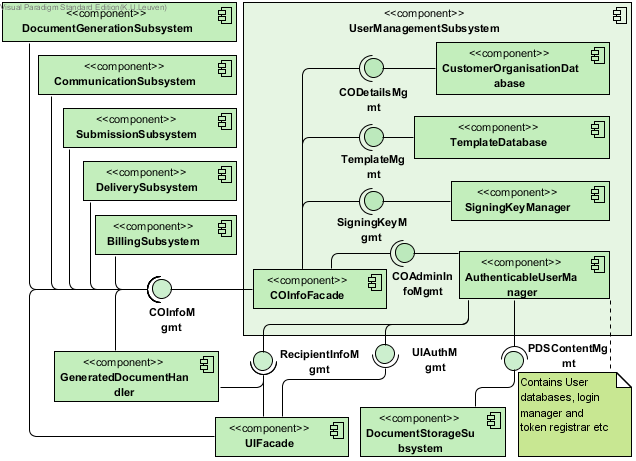
\includegraphics[width=\textwidth]{figures/User Managment Subsystem.png}
    \caption{Decomposition of \texttt{UserManagementSubsystem}}\label{fig:decomp-usersub}
\end{figure}

Describe the decomposition of \texttt{ComponentX} and how this relates to the
requirements.

\subsection{ZoomitDeliveryChannel}
\begin{figure}[!htp]
    \centering
    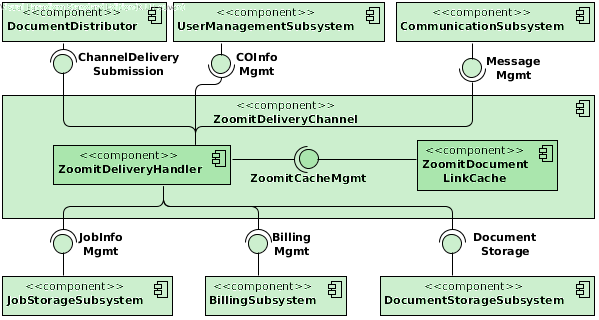
\includegraphics[width=\textwidth]{figures/ZoomitDeliveryChannel.png}
    \caption{Decomposition of \texttt{ZoomitDeliveryChannel}}\label{fig:decomp-zoomitchan}
\end{figure}

Describe the decomposition of \texttt{ComponentX} and how this relates to the
requirements.